\chapter{Results}
%Results:
%	-Total active days pre+post-trimming
%	-Total count of sp events (also pre+post?)
%-Overall detection rate pattern in all species
%-Overall activity pattern in all species
%(-Density curves throughout the year, obs per (week/month)) %Don't think so
%-Intro to how each sp will be presented



There were a total of $18 133$ active camera trapping days, which were unevenly distributed between the different period types (see figure \ref{fig:events}b). Filtering out time lapses and photos of nothing, there were $10 600$ triggers of the CTs. 
Of the nine most common wild species, there were a total of 5 844 independent events. Figure \ref{fig:events}a shows the total events of each species, and how the trimming of the data affected the count.

The type of CT flash had an overall minor effect on detection rates. 
The three least common species (lynx, pine marten and red deer) had the most variation explained by type of period and time since deployment (ie. highest marginal R2), as shown in table \ref{r2}, suggesting the high fit of fixed effect to be due to low sample sizes.
Most of the explained variation in detection rate was due to seasonal changes and variation between the different camera sites captured in the random terms. %The higher the st.dev in random effects, the more variation they will explain
For most species, the control periods (which never had white flashes) had a somewhat lower detection rate than the IR and white LED periods.
Diel patterns were consistent between all three types of periods.



I here present detailed results of all the nine mammalian species included in my analyses, grouped by taxonomic relationship.
Each species is presented with a photo taken by a white LED CT, 
a figure showing seasonal varitation in activity across time of day, 
a plot of the marginal means of the fixed effects in the GLMM model, showing the detection rates of all three types of periods (Control, IR and white LED) along a time axis,
and effect sizes in an equivalence test, 

%%% Figures %%%%%%%%%%%%%%%%%%%%%%%%%%%%%%%%%%%%%%%%%%%%%%%%%%%%%%

\begin{figure}
	\centering
	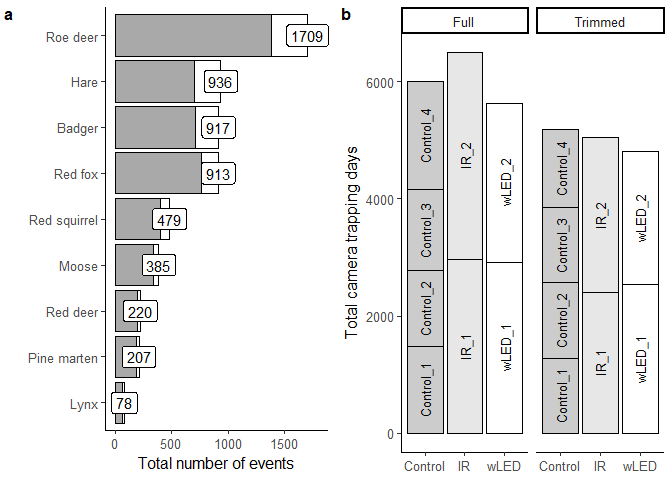
\includegraphics[width=\textwidth]{../R/glmm_sp_files/figure-html/days-count-2.png} 
		\caption[Camera trapping days and number of events]%
	{Trapping days and events, before and after trimming the data. a) Total number of events per species. Grey area marks the number of events that were included in the modelling. b) Total number of active camera days per period type. Trimming the data evened out the disproportions between period types.}\label{fig:events}
\end{figure}


\begin{table}[h]
	\centering
	\caption[Model performance]%AM: for hvilken modell?
	{Performance of species specific models \footnotesize \\
	Conditional R2 is a measure of how much variation was explained by both random and fixed effects, ranging from 0 to 1. Marginal R2 is for the fixed effects alone, and somewhere between 0.10 and 0.01 is considered good. Week of the year and site ID were used as random effects. The larger their standard deviations, the more variation in the data they can explain. Only sites that observed a species at least once were included in the model of said species.}\label{r2}
\begin{tabular}{lccccc}
	\toprule
	&\multicolumn{2}{c}{\bfseries Explained variation} & \multicolumn{3}{l}{\bfseries Standard deviations of random effects }	\\
Species & R2 (marg.) & R2 (cond.) & Week of the year & Site ID & N sites \\
	\midrule
    Lynx        & 0.060 & 0.18 & 0.52 & 0.68 & 22 \\  %22 sites  
    Pine marten & 0.052 & 0.22 & 0.72 & 0.74 & 42 \\  %42 sites
    Red deer    & 0.011 & 0.20 & 0.51 & 0.85 & 26 \\  %26 sites
 Red squirrel   & 0.010 & 0.30 & 0.81 & 1.03 & 37 \\  %37 sites
    Badger      & 0.006 & 0.39 & 1.27 & 1.01 & 48 \\  %48 sites
    Moose       & 0.004 & 0.19 & 0.73 & 0.63 & 41 \\  %41 sites
    Roe deer    & 0.003 & 0.38 & 0.56 & 1.29 & 47 \\  %47 sites
 Mountain hare  & 0.003 & 0.33 & 0.70 & 1.15 & 45 \\  %45 sites
    Red fox	    & 0.001 & 0.19 & 0.27 & 0.87 & 53 \\  %53 sites
    
    
 \bottomrule
\end{tabular}
\end{table}

%%% Tables %%%%%%%%%%%%%%%%%%%%%%%%%%%%%%%%%%%%%%%%%%%%%%%%%%%%%%

\clearpage

\begin{table}[ht]  % må inn for å fjerna begin{table} kvar gong tabellen oppdaterast!
\caption[Model results]
{ \footnotesize 
Results of Poisson mixed effects models on detection rate of species at 56 different locations in southeastern Norway, with three different treatment levels interacting with time since deployment (Time); periods from control sites (Intercept), periods with only IR camera (IR), periods with an additional white LED camera (wLED). Second Generation P-Values (SGPV) is identical to the proportion of a parameter that is inside the Region of Practical Equivalence (ROPE) in an equivalence test. Random effects were location ID and week of year. %TODO random effects st.dev.
%95\% Confidence Intervals and p-values were computed using the Wald approximation.
}
\label{tab:param}
\footnotesize
% latex table generated in R 4.0.4 by xtable 1.8-4 package
% Fri Mar 26 20:35:32 2021
\centering
{\tiny\renewcommand{\arraystretch}{.8}
	\resizebox{!}{.35\paperheight}{%
		\begin{tabular}[c]{llrlcrrr}
  \toprule
Species & Parameter & Coefficient & SE & 95\% CI & z & p & SGPV \\ 
\midrule
Roe deer & Intercept & -2.85 & 0.38 & (-3.58, -2.11) & -7.57 & $<$ .001 & 0.00 \\ 
& Time & -0.05 & 0.02 & (-0.09, -0.01) & -2.24 & \textbf{0.025}  & \textit{1.00} \\ 
& IR & -0.26 & 0.44 & (-1.12,  0.60) & -0.59 & 0.557  & 0.14 \\ 
& wLED & -0.13 & 0.44 & (-0.99,  0.73) & -0.30 & 0.761  & 0.14 \\ 
& Time * IR & 0.02 & 0.03 & (-0.04,  0.08) & 0.71 & 0.476  & \textit{1.00} \\ 
& Time * wLED & $<$ 0.01 & 0.03 & (-0.05,  0.06) & 0.12 & 0.901  & \textit{1.00} \\ 
\midrule
Moose & Intercept & -4.15 & 0.30 & (-4.75, -3.56) & -13.75 & $<$ .001 & 0.00 \\ 
& Time & $<$ 0.01 & 0.05 & (-0.08,  0.10) & 0.14 & 0.890  & \textit{1.00} \\ 
& IR & 		-0.08 & 0.35 & (-0.77,  0.60) & -0.23 & 0.814  & 0.17 \\ 
& wLED & 	 0.30 & 0.34 & (-0.36,  0.97) & 0.89 & 0.373  & 0.18 \\ 
& Time * IR & 0.05 & 0.06 & (-0.06,  0.17) & 0.86 & 0.389  & 0.75 \\ 
& Time * wLED & $<$ 0.01 & 0.06 & (-0.12,  0.10) & -0.12 & 0.902  & \textit{1.00} \\ 
\midrule
Red deer & Intercept & -3.89 & 0.41 & (-4.69, -3.09) & -9.55 & $<$ .001 & 0.00 \\ 
& Time & -0.09 & 0.06 & (-0.21,  0.02) & -1.63 & 0.104  & 0.53 \\ 
& IR & $<$ 0.01 & 0.50 & (-0.99,  0.97) & -0.02 & 0.984  & 0.12 \\ 
& wLED & -0.69 & 0.53 & (-1.72,  0.35) & -1.30 & 0.192  & 0.12 \\ 
& Time * IR & 0.06 & 0.08 & (-0.09,  0.21) & 0.81 & 0.421  & 0.65 \\ 
& Time * wLED & 0.23 & 0.08 & ( 0.08,  0.38) & 2.96 & \textbf{0.003}  & 0.00 \\ 
\midrule
Badger & Intercept & -4.49 & 0.37 & (-5.22, -3.76) & -12.12 & $<$ .001 & 0.00 \\ 
& Time & 0.06 & 0.03 & ( 0.00,  0.13) & 1.85 & 0.064  & 0.82 \\ 
& IR & 0.17 & 0.39 & (-0.59,  0.93) & 0.44 & 0.657  & 0.16 \\ 
& wLED & 0.24 & 0.38 & (-0.51,  0.99) & 0.64 & 0.523  & 0.16 \\ 
& Time * IR & 0.01 & 0.04 & (-0.07,  0.09) & 0.27 & 0.784  & \textit{1.00} \\ 
& Time * wLED & $<$ 0.01 & 0.04 & (-0.07,  0.08) & 0.11 & 0.914  & \textit{1.00} \\ 
\midrule
Pine Marten & Intercept & -5.95 & 0.54 & (-7.02, -4.89) & -10.95 & $<$ .001 & 0.00 \\ 
& Time & 0.09 & 0.09 & (-0.09,  0.28) & 0.97 & 0.331  & 0.52 \\ 
& IR & 1.69 & 0.58 & ( 0.55,  2.82) & 2.92 & \textbf{0.004}  & 0.00 \\ 
& wLED & 0.76 & 0.61 & (-0.43,  1.95) & 1.25 & 0.210  & 0.10 \\ 
& Time * IR & -0.11 & 0.11 & (-0.32,  0.09) & -1.07 & 0.286  & 0.46 \\ 
& Time * wLED & 0.03 & 0.11 & (-0.18,  0.24) & 0.30 & 0.768  & 0.56 \\ 
\midrule
Red fox & Intercept & -3.44 & 0.26 & (-3.94, -2.94) & -13.40 & $<$ .001 & 0.00 \\ 
& Time & $<$ 0.01 & 0.03 & (-0.06,  0.05) & -0.02 & 0.985  & \textit{1.00} \\ 
& IR & 0.03 & 0.32 & (-0.59,  0.65) & 0.09 & 0.926  & 0.19 \\ 
& wLED & 0.18 & 0.31 & (-0.44,  0.79) & 0.56 & 0.574  & 0.19 \\ 
& Time * IR & $<$ 0.01 & 0.04 & (-0.08,  0.07) & -0.06 & 0.949  & \textit{1.00} \\ 
& Time * wLED & -0.01 & 0.04 & (-0.08,  0.06) & -0.30 & 0.763  & \textit{1.00} \\ 
\midrule
Lynx & Intercept & -4.82 & 0.58 & (-5.96, -3.67) & -8.24 & $<$ .001 & 0.00 \\ 
& Time & -0.22 & 0.14 & (-0.49,  0.05) & -1.58 & 0.113  & 0.24 \\ 
& IR & -0.20 & 0.72 & (-1.61,  1.21) & -0.28 & 0.781  & 0.08 \\ 
& wLED & 0.15 & 0.72 & (-1.26,  1.55) & 0.20 & 0.839  & 0.08 \\ 
& Time * IR & 0.25 & 0.16 & (-0.07,  0.57) & 1.53 & 0.127  & 0.22 \\ 
& Time * wLED & 0.26 & 0.16 & (-0.06,  0.58) & 1.59 & 0.112  & 0.20 \\ 
\midrule
Hare & Intercept & -3.91 & 0.36 & (-4.61, -3.21) & -10.94 & $<$ .001 & 0.00 \\ 
& Time & 0.04 & 0.03 & (-0.03,  0.10) & 1.12 & 0.263  & \textit{1.00} \\ 
& IR & 0.38 & 0.42 & (-0.44,  1.21) & 0.91 & 0.363  & 0.14 \\ 
& wLED & 0.25 & 0.42 & (-0.58,  1.08) & 0.59 & 0.555  & 0.14 \\ 
& Time * IR & -0.05 & 0.04 & (-0.13,  0.03) & -1.26 & 0.209  & 0.88 \\ 
& Time * wLED & $<$ 0.01 & 0.04 & (-0.08,  0.08) & 0.03 & 0.975  & \textit{1.00} \\ 
\midrule
Red squirrel & Intercept & -4.82 & 0.41 & (-5.63, -4.00) & -11.63 & $<$ .001 & 0.00 \\ 
& Time & 0.08 & 0.05 & (-0.01,  0.18) & 1.67 & 0.095  & 0.62 \\ 
& IR & 0.91 & 0.47 & (-0.02,  1.83) & 1.93 & 0.054  & 0.00 \\ 
& wLED & 0.61 & 0.48 & (-0.32,  1.54) & 1.28 & 0.201  & 0.13 \\ 
& Time * IR & -0.17 & 0.06 & (-0.29, -0.05) & -2.85 & \textbf{0.004}  & 0.13 \\ 
& Time * wLED & -0.02 & 0.06 & (-0.13,  0.10) & -0.29 & 0.771  & 0.92 \\ 
   \bottomrule
\end{tabular}}}

%IMR:
% Få med hvilke random effects du har brukt, og før opp stdev for disse. 
%Kanskje markere signifikante effekter med bold eller kursiv, for å lette lesingen?
\end{table}

\pagestyle{empty} %to remove page numbers from table page
%

\begin{figure}
		\begin{subfigure}{.5\textwidth}
		  \centering
		  	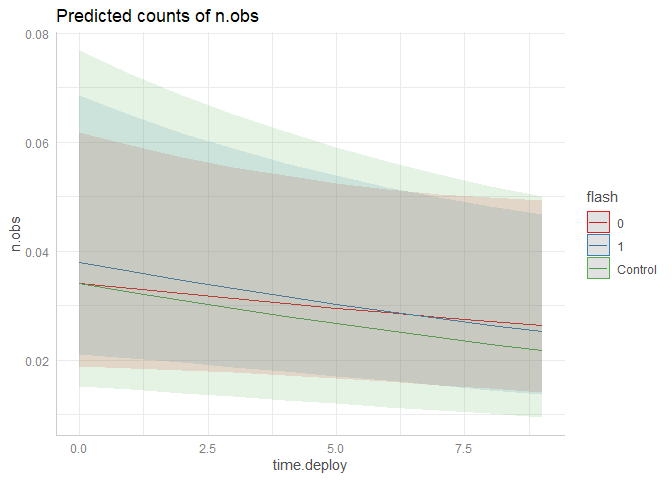
\includegraphics[width=.8\linewidth]{../R/glmm_sp_files/figure-gfm/raadyr-C-report-1.png}
		  \caption{Roe deer}
		  	\label{fig:glmm_raa}
	\end{subfigure}
		\begin{subfigure}{.5\textwidth}
		  \centering
		  	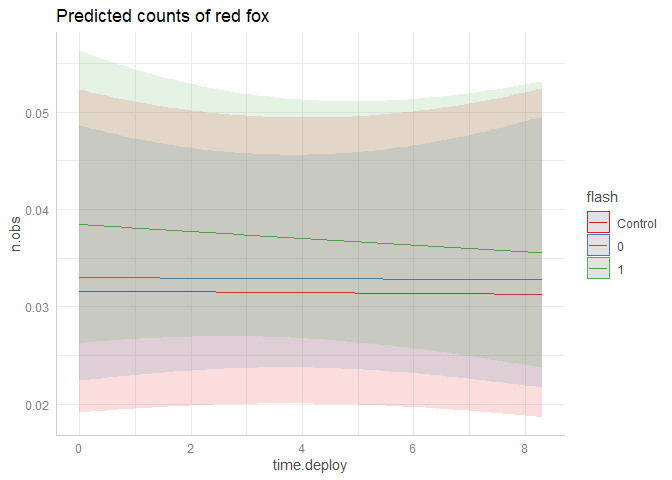
\includegraphics[width=.8\linewidth]{../R/glmm_sp_files/figure-gfm/rev-report-1.png}
		  \caption{Red fox}
		  	\label{fig:glmm_rev}
	\end{subfigure}
		\begin{subfigure}{.5\textwidth}
		  \centering
		  	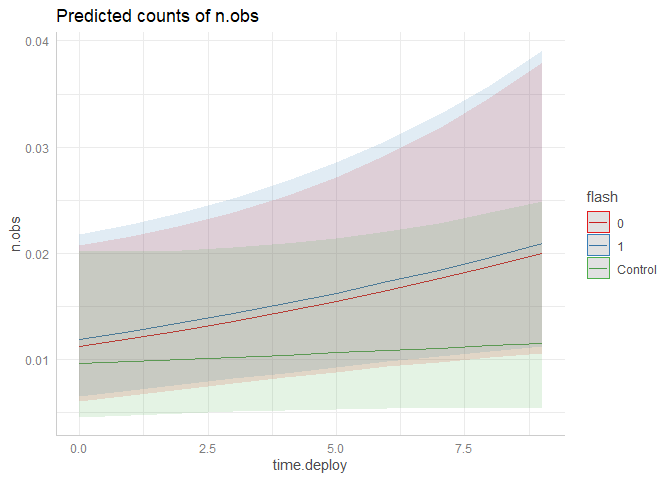
\includegraphics[width=.8\linewidth]{../R/glmm_sp_files/figure-gfm/grevling-report-1.png}
		  \caption{Badger}
		  	\label{fig:glmm_grvl}
	\end{subfigure}
		\begin{subfigure}{.5\textwidth}
		  \centering
		  	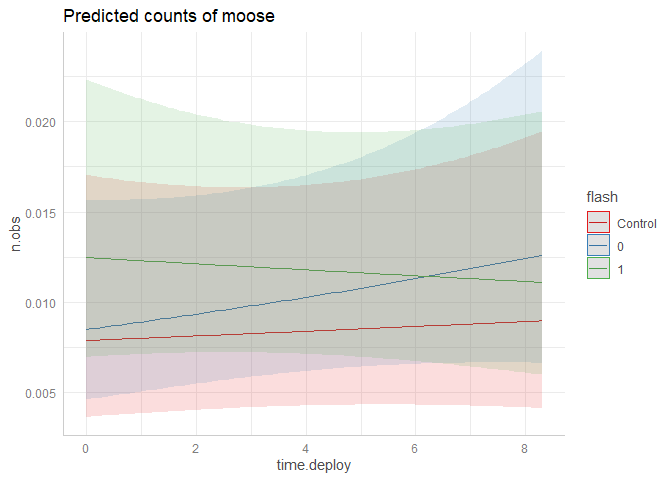
\includegraphics[width=.8\linewidth]{../R/glmm_sp_files/figure-gfm/elg-report-1.png}
		  \caption{Moose}
		  	\label{fig:glmm_elg}
	\end{subfigure}
		\begin{subfigure}{.5\textwidth}
		  \centering
		  	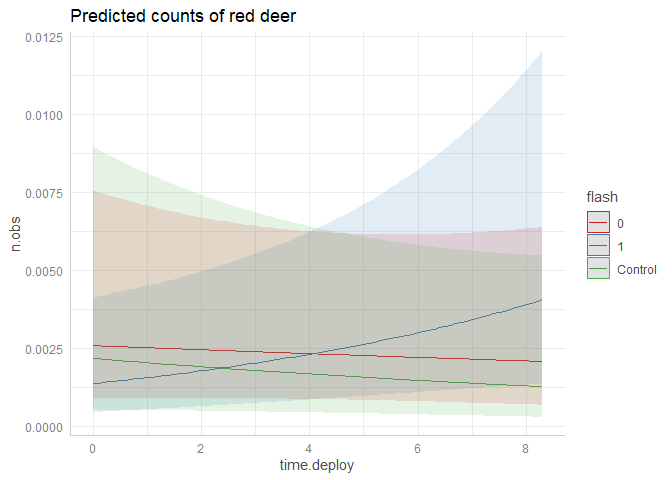
\includegraphics[width=.8\linewidth]{../R/glmm_sp_files/figure-gfm/hjort-report-1.png}
		  \caption{Red deer}
		  	\label{fig:glmm_hjort}
	\end{subfigure}
		\begin{subfigure}{.5\textwidth}
		  \centering
		  	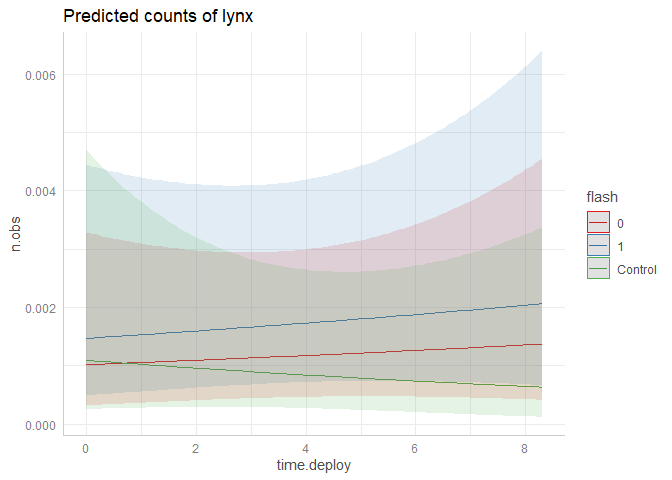
\includegraphics[width=.8\linewidth]{../R/glmm_sp_files/figure-gfm/gaupe-report-1.png}
		  \caption{Lynx}
		  	\label{fig:glmm_gaup}
	\end{subfigure}
		\caption{Fitted GLMM model to each species}
	\label{fig:glmm_sp}
\end{figure}



\begin{figure}
		\begin{subfigure}{.4\textwidth}
		  \centering
	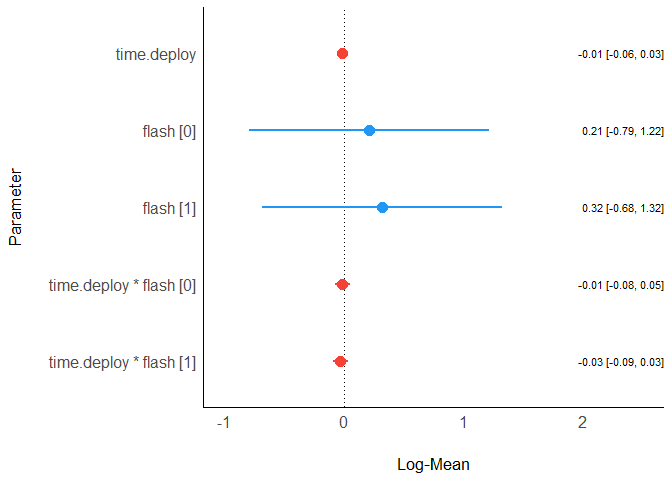
\includegraphics[scale=.4]{../R/glmm_sp_files/figure-gfm/parameters-1.png}
\caption{Intercept included}
		\label{fig:para_raa1}
	\end{subfigure}
		\begin{subfigure}{.4\textwidth}
		  \centering
	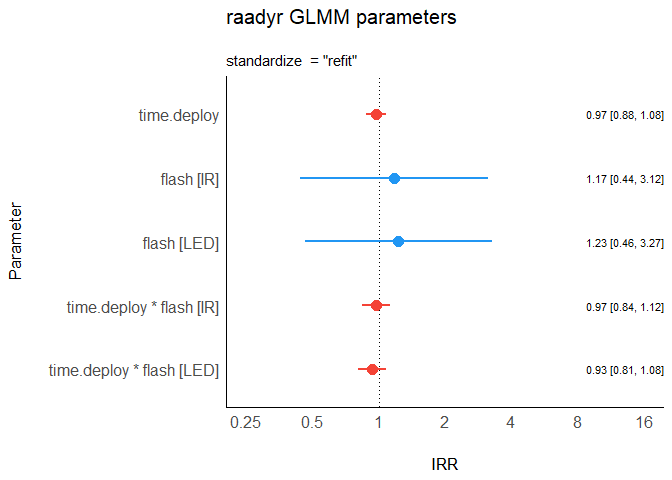
\includegraphics[scale=.4]{../R/glmm_sp_files/figure-gfm/parameters-2.png}
\caption{with values printed}
		\label{fig:para_raa2}
	\end{subfigure}
		\begin{subfigure}{.8\textwidth}
		  \centering
	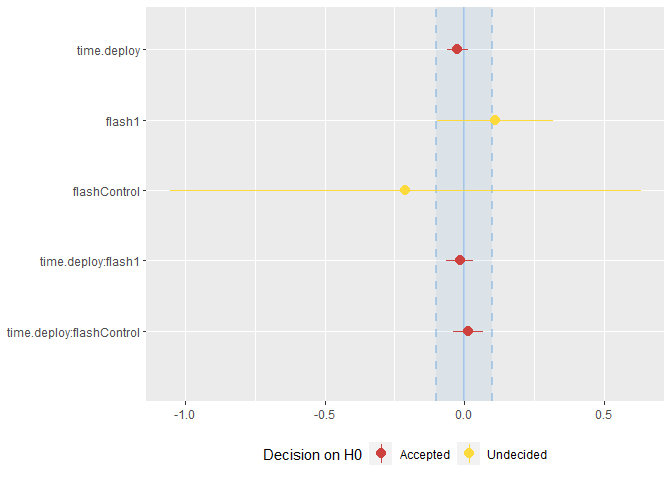
\includegraphics[scale=1]{../R/glmm_sp_files/figure-gfm/parameters-3.png}
\caption{Equivalence test}
		\label{fig:para_raa3}
	\end{subfigure}
		\caption{Visualising model parameters}
	\label{fig:para_sp}
\end{figure}


%%%%%%%%%%%%%%%%%%%%%%%%%%%%%%%%%%%%%%%%%%%%%%%%%%%%%%%%%%%%%%%%%%%%

\clearpage %to force the insertion of parameters table
\pagestyle{fancy} %to return to fancy pagestyle
\section{Cervidae}
Three species of the family Cervidae, namely roe deer, moose and red deer, were detected.
All three cervids were detected throughout the day, but had pronounced bimodal peaks around the twilight hours. % showed a crepuscular activity pattern, ie. that they were mainly active during the twilight hours.
However, during winter, roe deer shifted towards a more diurnal pattern, as seen in figure \ref{raadyr}a. 
On the other hand, moose (figure \ref{elg}) and red deer (figure \ref{hjort}) showed a crepuscular pattern throughout the year.
Consequently, all cervids were subject to the white flash during twilight and night. %although a large proportion of roe deer detections happened during daylight.

Roe deer had the highest detection rates in the study. Moose and red deer had similar detection rates at the sites where they were present, but moose were detected at more sites.
Roe deer and red deer had significant responses to any model parameters in a standard null hypothesis significance test (NHST). During white LED periods there was a significant increase in red deer detection rates along the time axis (p = 0.003). However, white LED periods weren't significantly different from IR periods, as they had a large overlap of confidence intervals. 

For roe deer, the control period had a significantly negative trend along the time axis. However, the equivalence test deemed it practically equivalent to having no effect, as it was completely inside the ROPE. The slopes of the IR periods and white LED periods were also found practically equivalent to zero effect (ie. Second Generation P-Value of 100\%).

The moose also had no trend along the time axis during control periods, but although the SGPV for Time * wLED were 100\%, the equivalence test failed to decide %NHT: Failed to decide? Kunne ikke testen avgjøre om H0 skulle beholdes eller forkastes?
on the parameter’s practical equivalence. %foreløpig løysing på NHT sitt spørsmål  


%%% Figures %%%%%%%%%%%%%%%%%%%%%%%%%%%%%%%%%%%%%%%%%%%%%%%%%%%%%%
\begin{figure}[b]
\centering
	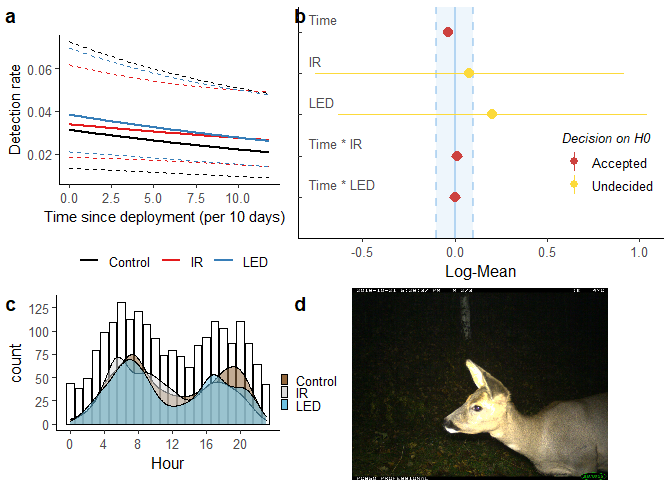
\includegraphics[width=13cm]{../R/glmm_sp_files/figure-html/parameters-1.png}
\caption[Roe deer]
{\footnotesize %\par
a) Bars represent the raw count of total roe deer detections per hour of the day, and density curves show the diel pattern for each season.
b) LED-CT photograph of a roe deer. This deer passed the camera repeatedly and often stopped in front of the flashing light.
c) Equivalence test of model parameters. 90\% confidence intervals are tested against the Region of Practical Equivalence (set to $\pm$0.1 Log-Mean).
d) The predicted detection rate of roe deer for each period type. 95\% confidence intervals are represented by dotted lines.}
\label{raadyr}
\end{figure}

\begin{figure}
		  \centering
	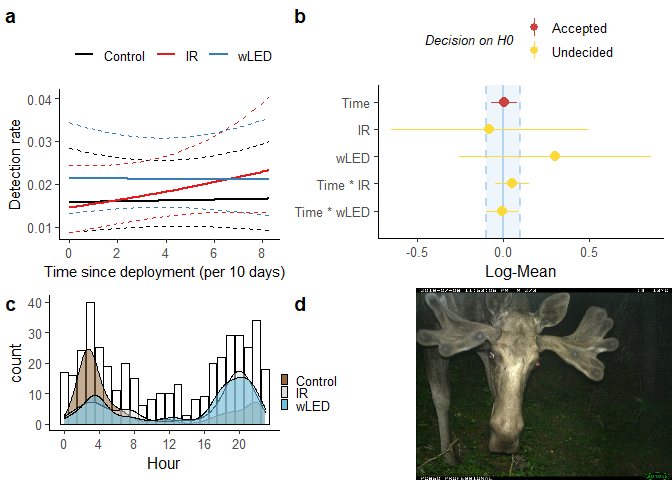
\includegraphics[width=13cm]{../R/glmm_sp_files/figure-html/elg2-1.png}
\caption[Moose]
{\footnotesize
	a) Bars represent the raw count of total moose detections per hour of the day, and density curves show the diel pattern for each season.
	b) LED-CT photograph of a moose. This bull foraged in front of the flash for a minute.
	c) Equivalence test of model parameters. 90\% confidence intervals are tested against the Region of Practical Equivalence (set to $\pm$0.1 Log-Mean).
	d) The predicted detection rate of moose for each period type. 95\% confidence intervals are represented by dotted lines.}
\label{elg}
\end{figure}

\begin{figure}
		  \centering
	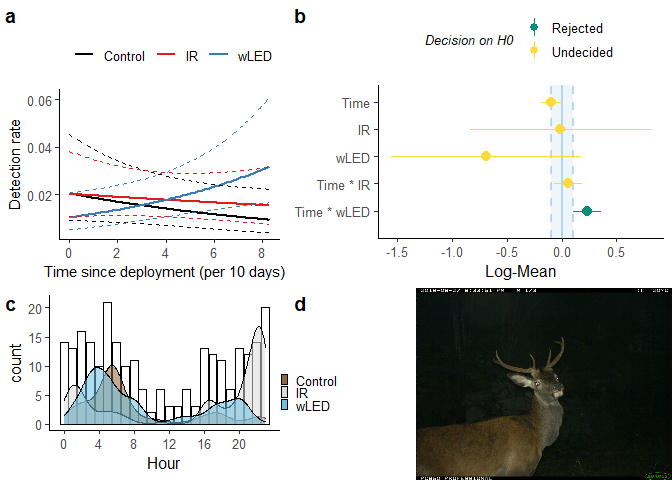
\includegraphics[width=13cm]{../R/glmm_sp_files/figure-html/hjort2-1.png}
\caption[Red deer]
{\footnotesize
	a) Bars represent the raw count of total red deer detections per hour of the day, and density curves show the diel pattern for each season.
	b) LED-CT photograph of a red deer. This stag stopped in front of the flash for a minute, observing the CTs intently, before moving on. Red deer were subsequently redetected several times during the same period.
	c) Equivalence test of model parameters. 90\% confidence intervals are tested against the Region of Practical Equivalence (set to $\pm$0.1 Log-Mean).
	d) The predicted detection rate of red deer for each period type. 95\% confidence intervals are represented by dotted lines.}
\label{hjort}
\end{figure}
%%%%%%%%%%%%%%%%%%%%%%%%%%%%%%%%%%%%%%%%%%%%%%%%%%%%%%%%%%%%%%%%%%%%%

\clearpage
\section{Carnivora}
Four of the most commonly detected species were from the order Carnivora, split by the three families Mustelidae, Canidae and Felidae. 
Badgers showed a clear nocturnal activity pattern, and was most active during spring, as seen in figure \ref{grevling}a. 
The other three species showed a crepuscular pattern, having activity peaks around the twilight hours.
Both foxes (figure \ref{rev}) and pine martens (figure \ref{maar}) had clear peaks at dusk. Martens were increasingly active during the summer, whilst foxes remained almost identical in activity the whole year through. In fact, foxes had the lowest variation in seasonal pattern overall, which is represented by the low standard deviation in week of the year in table 3.1.
The lynx was the least common of the nine species included in my analyses, with 78 events on 22 of the 56 sites. Accordingly, the density curves in figure \ref{gaupe}a were quite rugged. Nevertheless, all peaks coincided well with the twilight hours of the respective seasons, and the summer had fewest total detections.
All carnivores were subject to the white LED during twilight and night time.

%Detection rates
Badgers and red foxes had third and fourth highest detection rates, whilst pine marten and lynx had the lowest detection rates.
%Significance test
Pine marten was the only carnivore with a significant parameter in a standard NHST. During IR periods the pine marten detection rates were significantly higher than that of control periods, but the difference between IR and white LED periods were non-significant.
% Equivalence test
For both badger and red fox, the treatment groups' trends along the time axis were practically identical to that of the control periods. Hence, the equivalence tests accepted the null hypothesis of no effect for those two species.

% Badger: Time parameter acted strange in equivalence test as it is rejected as identical to H0, although 82% of the CI is inside the ROPE. Also, the parameter isn't considered significant in an NHST (p = 0.064). I don't understand why it's green.


%%% Figures %%%%%%%%%%%%%%%%%%%%%%%%%%%%%%%%%%%%%%%%%%%%%%%%%%%%%%
\begin{figure}[b]
	\centering
	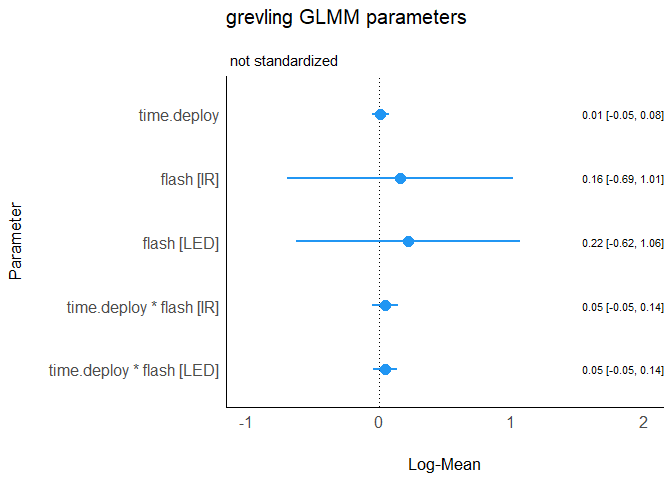
\includegraphics[width=13cm]{../R/glmm_sp_files/figure-html/grevling2-1.png}
	\caption[Badger]
	{\footnotesize
		a) Bars represent the raw count of total badger detections per hour of the day, and density curves show the diel pattern for each season.
		b) LED-CT photograph of a badger. This badger was foraging during rain weather, and showed no reaction to the white flash.
		c) Equivalence test of model parameters. 90\% confidence intervals are tested against the Region of Practical Equivalence (set to $\pm$0.1 Log-Mean).
		d) The predicted detection rate of badgers for each period type. 95\% confidence intervals are represented by dotted lines.}
	\label{grevling}
\end{figure}

\begin{figure}
	\centering
	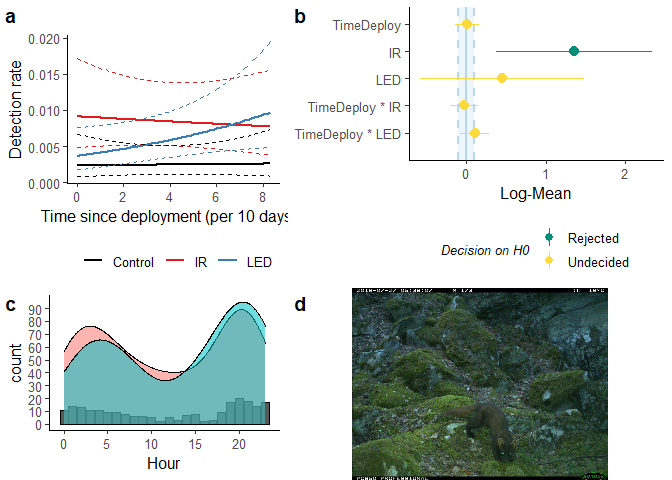
\includegraphics[width=13cm]{../R/glmm_sp_files/figure-html/maar2-1.png}
	\caption[Pine marten]
	{\footnotesize
		a) Bars represent the raw count of total pine marten detections per hour of the day, and density curves show the diel pattern for each season.
		b) LED-CT photograph of a pine marten. This marten defecated while observing the camera traps, then went on inspecting the area.
		c) Equivalence test of model parameters. 90\% confidence intervals are tested against the Region of Practical Equivalence (set to $\pm$0.1 Log-Mean).
		d) The predicted detection rate of martens for each period type. 95\% confidence intervals are represented by dotted lines.}
	\label{maar}
\end{figure}

\begin{figure}
		  \centering
	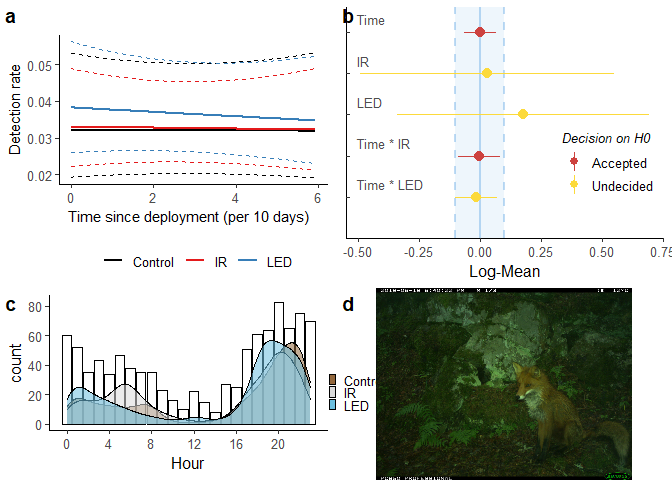
\includegraphics[width=13cm]{../R/glmm_sp_files/figure-html/rev2-1.png}
\caption[Red fox]
{\footnotesize
	a) Bars represent the raw count of total fox detections per hour of the day, and density curves show the diel pattern for each season.
	b) LED-CT photograph of a red fox. This fox stopped in front of the flashing camera and scratched its ear, before moving on. A second fox followed right behind.
	c) Equivalence test of model parameters. 90\% confidence intervals are tested against the Region of Practical Equivalence (set to $\pm$0.1 Log-Mean).
	d) The predicted detection rate of foxes for each period type. 95\% confidence intervals are represented by dotted lines.}
\label{rev}
\end{figure}

\begin{figure}
	\centering
	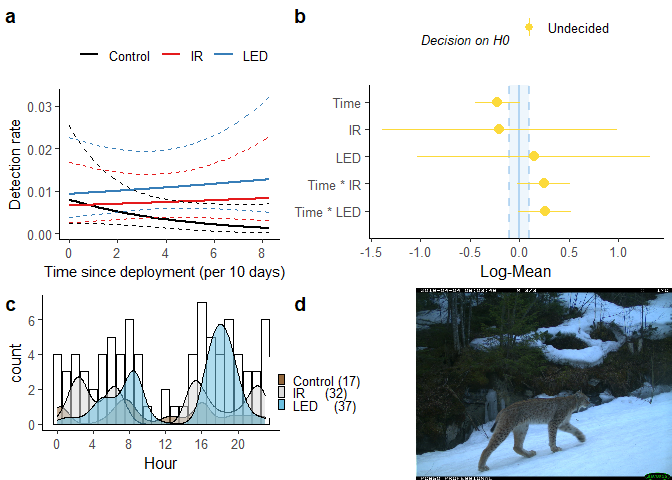
\includegraphics[width=13cm]{../R/glmm_sp_files/figure-html/gaupe2-1.png}
	\caption[Lynx]
	{\footnotesize
		a) Bars represent the raw count of total lynx detections per hour of the day, and density curves show the diel pattern for each season.
		b) LED-CT photograph of a lynx. This lynx stopped to observe the CTs, before moving on.
		c) Equivalence test of model parameters. 90\% confidence intervals are tested against the Region of Practical Equivalence (set to $\pm$0.1 Log-Mean). 
		d) The predicted detection rate of lynx for each period type. 95\% confidence intervals are represented by dotted lines.}
	\label{gaupe}
\end{figure}

%%%%%%%%%%%%%%%%%%%%%%%%%%%%%%%%%%%%%%%%%%%%%%%%%%%%%%%%%%%%%%%%%%%


\section{Glires}
The final two species in study both belong to the clade Glires, which consists of the two orders Rodentia (red squirrel) and lagomorphs (mountain hare). %wiki/Leporidae
%Diel patterns for seasons
The two Glires species were polar opposites in their diel patterns. Hares showed a nocturnal to crepuscular pattern, whereas squirrels were diurnal, and were never observed around midnight.
Like badgers, mountain hares were markedly more active during during the spring.
On the other hand, red squirrels were least detected during spring, and primarily from dawn untill midday. Long summer days allowed them to spread their activity between more sunlit hours, and peak detectability was during fall and winter.
	% were they flashed?
Therefore, out of these two species, only the hare was subject to white light during night, although squirrels sometimes passed a white LED CT during dawn.

% Detection rates (short)
Mountain hares had the second highest detection rates in the study, whilst red squirrels had similar detection rates to that of moose.
% Significance test
Nevertheless, the squirrel was the only Glires species that had any significant parameters in the standard NHST. IR periods had a significantly negative slope along the time axis than that of the control periods (p = 0.003), but they were not significantly different from the white LED periods. %AM: Som betyr?
% Equivalence test
The same was true for the equivalence test. Although IR periods were rejected as practically identical to the control periods, they weren't significantly different from white LED periods.
In other words, for squirrels, there seems to have been differences between the control sites and the treatment sites, but there were no significant differences between white LED and IR periods.



%%% Figures %%%%%%%%%%%%%%%%%%%%%%%%%%%%%%%%%%%%%%%%%%%%%%%%%%%%%%

\begin{figure}[b]
	\centering
	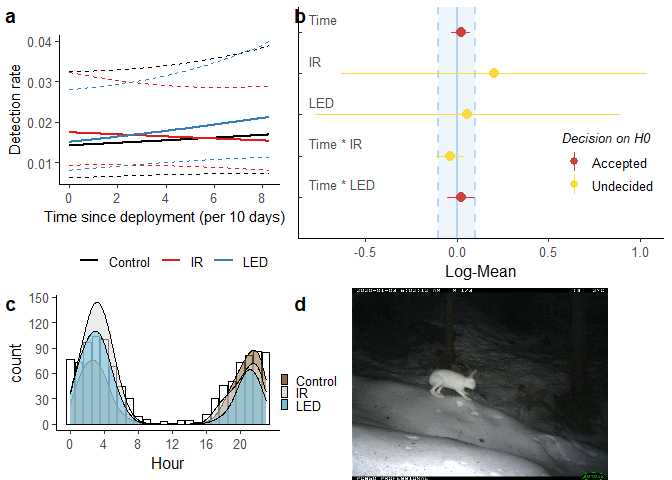
\includegraphics[width=13cm]{../R/glmm_sp_files/figure-html/hare2-1.png}
	\caption[Mountain hare]
	{\footnotesize
		a) Bars represent the raw count of total hare detections per hour of the day, and density curves show the diel pattern for each season.
		b) LED-CT photograph of a mountain hare in winter coat. This camera had repeated hare detections at night.
		c) Equivalence test of model parameters. 90\% confidence intervals are tested against the Region of Practical Equivalence (set to $\pm$0.1 Log-Mean). 
		d) The predicted detection rate of hares for each period type. 95\% confidence intervals are represented by dotted lines.}
	\label{hare}
\end{figure}

%\subsection{Red squirrel}

%Ultraviolet light is abundant during the day but not at night. There is a large increase in the ratio of ultraviolet to visible light in the morning and evening twilight hours. Many rodents are active during twilight hours (crepuscular activity), and UV-sensitivity would be advantageous at these times. Ultraviolet reflectivity is of dubious value for nocturnal rodents % wiki/Rodent 
\begin{figure}
	\centering
	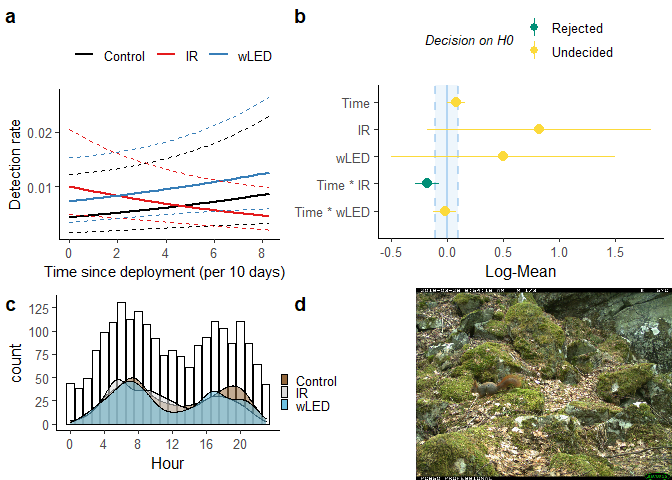
\includegraphics[width=13cm]{../R/glmm_sp_files/figure-html/ekorn2-1.png}
	\caption[Red squirrel]
	{\footnotesize
		a) Bars represent the raw count of total squirrel detections per hour of the day, and density curves show the diel pattern for each season.
		b) LED-CT photograph of a squirrel. Squirrels were seen at this site often, and the pine marten in figure \ref{maar} was seen sniffing around repeatedly during the same period.
		c) Equivalence test of model parameters. 90\% confidence intervals are tested against the Region of Practical Equivalence (set to $\pm$0.1 Log-Mean).
		d) The predicted detection rate of squirrels for each period type. 95\% confidence intervals are represented by dotted lines.}
	\label{ekorn}
\end{figure}

%%%%%%%%%%%%%%%%%%%%%%%%%%%%%%%%%%%%%%%%%%%%%%%%%%%%%%%%%%%%%%%%%%%%%







